\documentclass[10pt]{beamer}
\usetheme{metropolis}
\usecolortheme{default}

\usepackage{booktabs}
\usepackage{amsmath}
\usepackage{graphicx}
\usepackage{tikz}
\usetikzlibrary{arrows.meta, positioning}
\usepackage{multirow}
\usepackage{hyperref}

\title{The Median Voter Theorem}
\subtitle{ECO1028 - Politics Without Romance}
\author{Beatriz Gietner\\
\texttt{beatriz.gietner@dcu.ie}}
\date{\today}

\begin{document}

\maketitle

\begin{frame}{Outline}
\tableofcontents
\end{frame}


\section{Introduction: Why Do FF and FG Sound the Same?}

\begin{frame}{Before We Begin: A Diagnostic Question}
\textbf{Quick poll - think about Irish politics:}


On a left-right economic scale (1 = far left, 10 = far right):
\begin{itemize}
\item Where would you place Fianna Fáil?
\item Where would you place Fine Gael?
\item Where would you place yourself?
\end{itemize}



\alert{Common complaint:} "I can't tell the difference between FF and FG!"



\textbf{Today's question:} Is this convergence a bug or a feature of democracy?
\end{frame}

\begin{frame}{The Central Puzzle}
\href{http://www.nytimes.com/2010/02/07/business/economy/07view.html}{\alert{\textbf{Tyler Cowen (2010):}}}


\begin{quote}
"Any politician who strays too far from voters at the philosophical center will soon be out of office."
\end{quote}



\begin{quote}
"There is a dynamic that pushes politicians to embrace the preferences of the typical or `median' voter, who sits squarely in the middle of public opinion."
\end{quote}



\textbf{The Median Voter Theorem says:}
\begin{itemize}
\item In democratic competition, parties converge to the center
\item The median voter gets exactly what they want
\item FF ≈ FG might be what theory predicts!
\end{itemize}
\end{frame}

\begin{frame}[allowframebreaks]{A Simple Illustration: Picking a Restaurant}
\textbf{Al, Bob, and Charlie pick lunch by majority rule:}


\begin{itemize}
\item \textbf{Al} prefers: \alert{\$5.00} lunch
\item \textbf{Bob} prefers: \alert{\$10.00} lunch  
\item \textbf{Charlie} prefers: \alert{\$20.00} lunch
\end{itemize}



\textbf{Voting outcomes:}

\begin{table}
\centering
\small
\begin{tabular}{lcccc}
\toprule
\textbf{Options} & \textbf{Al} & \textbf{Bob} & \textbf{Charlie} & \textbf{Result} \\
\midrule
\$20 vs. \$5 & \$5 & \$5 & \$20 & \alert{\$5 wins} \\
\$10 vs. \$20 & \$10 & \$10 & \$20 & \alert{\$10 wins} \\
\$10 vs. \$5 & \$5 & \$10 & \$10 & \alert{\$10 wins} \\
\bottomrule
\end{tabular}
\end{table}



\alert{Pattern:} Bob (the median voter) always votes for the winner! \$10 beats any alternative.
\end{frame}

\begin{frame}[allowframebreaks]{From Restaurants to Elections}


\begin{center}
\includegraphics[width=0.85\textwidth]{restaurant_choice.png}
\end{center}

\textbf{Same logic applies to candidate competition:}

\small The median voter is the voter whose ideal point lies in the middle when preferences are ordered.


\textbf{If candidates can choose positions:}
\begin{itemize}
\item Each tries to get closer to median voter than opponent
\item If A positions left of median, B positions just right of median
\item Then A moves right to beat B...
\item This continues until...
\end{itemize}

\begin{center}
\includegraphics[width=0.9\textwidth]{convergence_dynamics.png}
\end{center}


\framebreak
\alert{\textbf{Equilibrium:}} Both candidates locate exactly at median voter's position!
\begin{itemize}
\item Both get ~50\% of votes
\item Median voter gets their ideal policy regardless of who wins
\end{itemize}



\textbf{Historical context:}
\begin{itemize}
\item Duncan Black (1948): First formal statement
\item Anthony Downs (1957): Applied to electoral competition
\end{itemize}
\end{frame}


\section{The Theory: Why the Median Wins}

\begin{frame}{The Key Assumption: Single-Peaked Preferences}
\begin{block}{Single-Peaked Preferences}
\textbf{Definition:} Preferences are single-peaked if:
\begin{itemize}
\item Alternatives can be ordered on a single dimension
\item Each voter has one ideal point (their "peak")
\item Utility declines moving away from ideal point in either direction
\end{itemize}
\end{block}



\textbf{Examples that work:}
\begin{itemize}
\item Tax rates (0\% to 100\%)
\item Education spending (\euro 0 to \euro X per student)
\item Left-right ideology
\end{itemize}

 \textbf{Examples that don't work:}
\begin{itemize}
\item Multidimensional choices (e.g. taxes \emph{and} immigration together)
\item Policy \emph{bundles} (packages that mix issues)
\item Issues with no shared left--right ordering across voters
\end{itemize}

\end{frame}

\begin{frame}[allowframebreaks]{Visual Proof: Why Median Beats Any Alternative}
\hypertarget{visual-proof}{}
\textbf{Five voters with different ideal points:}


\begin{center}
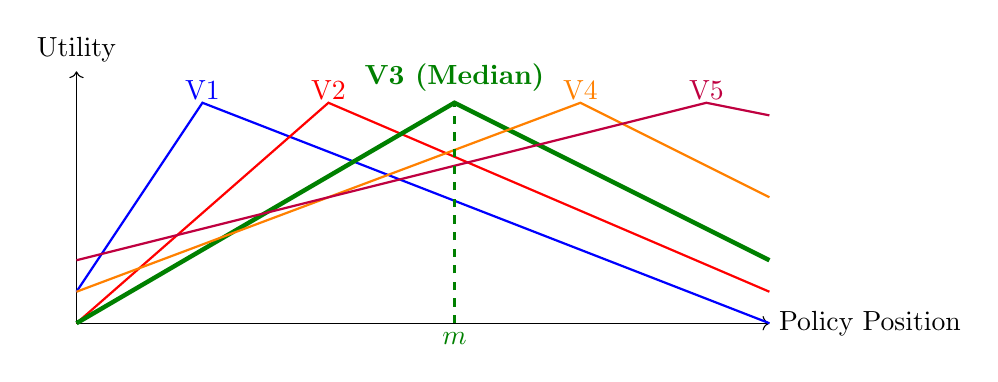
\begin{tikzpicture}[scale=0.8]

\draw[->] (0,0) -- (11,0) node[right] {Policy Position};
\draw[->] (0,0) -- (0,4) node[above] {Utility};


\draw[blue, thick] (0,0.5) -- (2,3.5) -- (11,0);
\node[blue] at (2,3.7) {V1};


\draw[red, thick] (0,0) -- (4,3.5) -- (11,0.5);
\node[red] at (4,3.7) {V2};


\draw[green!50!black, ultra thick] (0,0) -- (6,3.5) -- (11,1);
\node[green!50!black] at (6,3.9) {\textbf{V3 (Median)}};

\draw[orange, thick] (0,0.5) -- (8,3.5) -- (11,2);
\node[orange] at (8,3.7) {V4};

\draw[purple, thick] (0,1) -- (10,3.5) -- (11,3.3);
\node[purple] at (10,3.7) {V5};


\draw[green!50!black, dashed, thick] (6,0) -- (6,3.5);
\node[below, green!50!black] at (6,0) {$m$};
\end{tikzpicture}
\end{center}
\small Each curve shows a single-peaked ranking: utility is highest at the voter’s ideal point and falls as policy moves away.

\framebreak   

\textbf{The logic:}
\begin{itemize}
\item Voters 3, 4, 5 prefer $m$ to any proposal $< m$ (that's a majority: 3 out of 5)
\item Voters 1, 2, 3 prefer $m$ to any proposal $> m$ (also a majority: 3 out of 5)
\item \alert{$m$ defeats any alternative in pairwise vote!}
\end{itemize}


\small{\hyperlink{formal-proof}{\beamerbutton{See formal algebraic proof in Appendix A}}}
\end{frame}

\begin{frame}[allowframebreaks]{The Problem: Arrow and Majority Voting}
\small Arrow studied whether we can aggregate individual rankings into a consistent \emph{social} ranking.

\textbf{Arrow’s Impossibility Theorem (1951):}
 With three or more alternatives, no voting rule can satisfy all of the following:
\begin{itemize}
\item \textbf{Unanimity (Pareto axiom):}  
If everyone prefers $x$ to $y$, society must rank $x$ above $y$.

\item \textbf{Non-dictatorship:}  
No single voter always determines the social ranking.

\item \textbf{Independence of Irrelevant Alternatives (IIA):}  
The social ranking of $x$ versus $y$ depends only on how individuals rank $x$ versus $y$, not on other options.

\item \textbf{Unrestricted domain (Universality):}  
The rule must work for all possible individual preference orderings.
\end{itemize}

\framebreak


\textbf{What this means for majority voting:}
\begin{itemize}
\item Majority voting respects unanimity and is not a dictatorship
\item Arrow implies that transitivity of the social ranking cannot be guaranteed
\item Under majority voting, the failure shows up as \alert{non-transitivity} (cycles)
\item Cycles imply no stable social ranking
\item Outcomes can depend on the voting agenda
\end{itemize}
\end{frame}


\begin{frame}[allowframebreaks]{Arrow’s Axioms: Real-World Policy Example}

\textbf{Policy choices:}
\begin{itemize}
\item $x$ = High public spending on healthcare
\item $y$ = Low public spending on healthcare
\item $z$ = Large tax cuts instead
\end{itemize}



\textbf{Unanimity (Pareto axiom):}
\begin{itemize}
\item If every voter prefers high healthcare spending ($x$) to low spending ($y$),
\item then society should rank $x \succ y$.
\end{itemize}
\framebreak
\textbf{Non-dictatorship:}
\begin{itemize}
\item The outcome should not depend only on one powerful voter or politician.
\end{itemize}

\textbf{Independence of Irrelevant Alternatives (IIA):}
\begin{itemize}
\item The social ranking of high vs low healthcare spending ($x$ vs $y$)
\item should not change just because tax cuts ($z$) are added or removed from the ballot.
\end{itemize}

\textbf{Unrestricted domain:}
\begin{itemize}
\item The voting rule must handle all possible rankings of these policies,
\item including voters who prioritise tax cuts over healthcare.
\end{itemize}

\end{frame}


\begin{frame}{Condorcet Cycle (Majority Voting Can Loop)}

\textbf{Three groups of voters, three options $L, M, H$:}

\begin{center}
\small
\begin{tabular}{lccc}
\toprule
\textbf{Group (size)} & \textbf{1st} & \textbf{2nd} & \textbf{3rd} \\
\midrule
A (1/3) & $L$ & $H$ & $M$ \\
B (1/3) & $H$ & $M$ & $L$ \\
C (1/3) & $M$ & $L$ & $H$ \\
\bottomrule
\end{tabular}
\end{center}

\textbf{Pairwise majorities:}
\begin{itemize}
\item $L$ beats $H$ (A + C)
\item $H$ beats $M$ (A + B)
\item $M$ beats $L$ (B + C)
\end{itemize}

\alert{So: $L \succ H \succ M \succ L$ (no Condorcet winner).}

\end{frame}


\begin{frame}{The Intensity Problem}
\textbf{A fundamental feature (or bug?) of democracy:}


\begin{quote}
"Your vote counts the same whether you're passionate about an issue or completely indifferent."
\end{quote}



\begin{columns}
\begin{column}{0.48\textwidth}
\textbf{Markets:}
\begin{itemize}
\item "Dollar votes"
\item Can express intensity through willingness to pay
\item Efficient allocation
\end{itemize}
\end{column}


\begin{column}{0.48\textwidth}
\textbf{Voting:}
\begin{itemize}
\item One person, one vote
\item No intensity mechanism
\item Equal but potentially inefficient
\end{itemize}
\end{column}
\end{columns}

\end{frame}


\section{Application 1: Taxation and Inequality}

\begin{frame}{The Meltzer-Richard Model (1981)}
\textbf{Question:} Why do democracies redistribute income?



\textbf{Setup:}
\begin{itemize}
\item Society chooses tax rate $t$ (0 to 100\%)
\item Revenue redistributed equally to all citizens
\item Person $i$ with income $y_i$ receives: $(1-t)y_i + t \cdot \bar{y}$
\end{itemize}



\textbf{Key insight:}
\begin{itemize}
\item If your income $<$ average income: you benefit from redistribution
\item If your income $>$ average income: you lose from redistribution
\item The \alert{median voter's income} determines the tax rate
\end{itemize}
\end{frame}

\begin{frame}{Meltzer-Richard: The Prediction}
\textbf{Case 1: Low inequality ($y_{\text{median}} = \bar{y}$)}
\begin{itemize}
\item Median voter pays in exactly what they receive back
\item Redistribution is pure deadweight loss
\item \alert{Prediction:} $t = 0$ (no redistribution)
\end{itemize}



\textbf{Case 2: High inequality ($y_{\text{median}} < \bar{y}$)}
\begin{itemize}
\item Median voter earns less than average
\item Benefits from redistribution (net recipient)
\item Trade-off: redistribution benefit vs. deadweight loss
\item \alert{Prediction:} Positive tax rate, more redistribution
\end{itemize}



\alert{\textbf{Main Result:}} Greater inequality → larger gap between median and mean → median voter demands more redistribution → higher taxes and social spending
\end{frame}

\begin{frame}{Numerical Example}
\textbf{Example 1: Equal society}
\begin{itemize}
\item Incomes: €40k, €45k, €50k, €55k, €60k
\item Median = €50k, Mean = €50k
\item Median voter: no net benefit from redistribution
\item \alert{MVT prediction:} $t = 0$
\end{itemize}



\textbf{Example 2: Unequal society}
\begin{itemize}
\item Incomes: €20k, €30k, €40k, €60k, €100k
\item Median = €40k, Mean = €50k
\item At $t = 50\%$: Median gets $(0.5)(€40k) + (0.5)(€50k) = €45k$
\item That's €5k more than with no redistribution!
\item \alert{MVT prediction:} High tax rate, significant redistribution
\end{itemize}



\textbf{Empirical evidence:} Mixed. Positive relationship in some studies, weak in others. US puzzle: high inequality but small welfare state.
\end{frame}

\begin{frame}{Irish Context: Water Charges (2014-2016)}
\textbf{A recent test of median voter power:}

\begin{itemize}
\item 2014: Government introduces water charges (€60-€160/household)
\item Rationale: User-pays principle, fund infrastructure
\item \alert{Massive public opposition} (60-70\% opposed in polls)
\item Mass protests, non-payment campaigns
\item 2016: Charges suspended $\rightarrow$ 2017: Abolished
\end{itemize}

\textbf{MVT interpretation:}
\begin{itemize}
\item \textbf{Misjudgment:} Government assumed median voter was a "Fiscal Responsibility" voter.
\item \textbf{Reality:} Median voter was actually an "Anti-Austerity" voter.
\item \textbf{Result:} Electoral pressure forced reversal. (Median wins!)
\end{itemize}

\textbf{Question for Week 4 presentations:} Do Irish governments generally respond to median voter? Or was this exceptional?
\end{frame}


\section{Application 2: The Efficiency Problem}

\begin{frame}{Does Median Voter = Social Optimum?}
\begin{center}
\Large Does the median voter outcome produce \alert{efficient} results?
\end{center}




\textbf{In other words:}
\begin{itemize}
\item Markets (ideally) maximize total surplus
\item Does majority voting maximize social welfare?
\item When do median voter preferences = efficient outcome?
\end{itemize}




\alert{Spoiler:} Not always! Let's see a concrete example...
\end{frame}

\begin{frame}[allowframebreaks]{The Bridge Project}
\textbf{Setup:}
\begin{itemize}
\item Bridge would serve 10 people
\item 6 people value it at €50 each
\item 4 people value it at €100 each
\item Cost: €60 per person → Total cost = €600
\item Assume equal cost sharing (a head tax): each pays €60 if the bridge is built
\end{itemize}



\textbf{Median voter analysis:}
\begin{itemize}
\item Median value = €50 (6th person when ordered)
\item Median voter's net benefit = €50 - €60 = \alert{-€10}
\item \alert{Majority vote (6-4):} Bridge NOT built
\end{itemize}

\framebreak

\textbf{Efficiency analysis:}
\begin{itemize}
\item Total benefit = $(6)(€50) + (4)(€100) = €700$
\item Total cost = €600
\item Net social benefit = \alert{+€100}
\item \alert{Efficient outcome:} Bridge SHOULD be built
\end{itemize}



\alert{\textbf{Conclusion:}} Median voter rejects a socially beneficial project!
\end{frame}

\begin{frame}{When Does MVT Produce Efficiency?}
\textbf{The problem in the bridge example:}
\begin{itemize}
\item Preferences are \alert{skewed} (6 low-value, 4 high-value)
\item Median (€50) $\neq$ Mean (€70)
\item Median voter doesn't represent average benefit
\end{itemize}



\textbf{When can the median outcome be efficient?}
\begin{itemize}
\item In some symmetric settings, the median voter’s choice can coincide with the utilitarian optimum
\item In general, majority voting need not maximise total surplus (as the bridge example shows)
\end{itemize}




\textbf{Why can't we use better mechanisms?}
\begin{itemize}
\item Lindahl pricing: everyone pays their valuation → efficient
\item But: preference revelation problem (incentive to lie)
\item We're stuck with imperfect mechanisms
\end{itemize}
\end{frame}


\section{Challenges: Identity, Assumptions, and Polarization}

\begin{frame}{Challenge 1: Identity Matters - Indian Villages}
\textbf{Chattopadhyay \& Duflo (2004):}


\textbf{Setup:} India randomly assigned some villages to reserve chief position for women



\textbf{MVT prediction:}
\begin{itemize}
\item Same constituency → same median voter
\item Gender of leader shouldn't matter
\item Same policies regardless
\end{itemize}



\textbf{Finding:} \alert{Leaders invest in infrastructure matching their gender's needs}
\begin{itemize}
\item West Bengal: Women complain about water/roads → Female leaders invest more in water/roads
\item Rajasthan: Women complain about water (not roads) → Female leaders invest more in water, less in roads
\end{itemize}



\alert{\textbf{Lesson:}} Identity of leader matters, not just constituency! MVT is incomplete.
\end{frame}

\begin{frame}{Challenge 2: Party Matters - US Evidence}
\textbf{Same constituency, different parties = different votes:}



\textbf{US Senate (Poole \& Rosenthal 1996):}
\begin{itemize}
\item 2 senators per state = same constituency
\item When one is Democrat, one Republican: they vote very differently
\item Party $>$ Constituency
\end{itemize}



\textbf{US House Close Elections (Lee, Moretti, Butler 2004):}
\begin{itemize}
\item Regression discontinuity: 49.9\% vs 50.1\%
\item Virtually identical constituencies
\item \alert{Huge gap in voting records} (ADA scores differ by 60-80 points - ADA scores are a standard index of how liberal or conservative a U.S. legislator’s voting record is - $\uparrow$ score = + liberal)
\item Party identity $>$ Median voter
\end{itemize}



\alert{\textbf{Why?}} Party discipline, career incentives, primary electorates, ideological selection


\small{\hyperlink{evidence-against}{\beamerbutton{See detailed evidence in Appendix B}}}
\end{frame}

\begin{frame}{The Six Critical Assumptions}
\textbf{MVT assumes:}

\begin{enumerate}
\item \textbf{Single-dimensional voting}
\begin{itemize}
\item Reality: Economic + cultural + identity + globalization dimensions
\end{itemize}


\item \textbf{Only two candidates}
\begin{itemize}
\item Reality: Multi-party systems (Ireland's PR-STV!)
\end{itemize}


\item \textbf{No ideology} (pure office motivation)
\begin{itemize}
\item Reality: Politicians care about policy, not just winning
\end{itemize}


\item \textbf{No selective voting} (everyone votes)
\begin{itemize}
\item Reality: Base mobilization vs. median voter appeal trade-off
\end{itemize}


\item \textbf{No money in politics}
\begin{itemize}
\item Reality: Donors pull candidates to extremes
\end{itemize}


\item \textbf{Full information}
\begin{itemize}
\item Reality: Rational ignorance, polls are imperfect
\end{itemize}
\end{enumerate}



\alert{All six are violated to varying degrees. This explains deviations from MVT!}
\end{frame}

\begin{frame}{Modern Polarization: Has the Median Voter Lost Power?}
\href{https://www.ft.com/content/7ab73ad8-21ec-39f3-ab8d-a559a110d210}{\alert{\textbf{Diane Coyle (2015):}}}

\begin{quote}
"Why does the mainstream middle of the political spectrum appear to have been hollowed out, with extreme parties... doing well, and the greater polarisation of major parties?"
\end{quote}



\textbf{Evidence: US polarization (1880-present)}
\begin{itemize}
\item 1970s: Peak MVT era - parties overlapped
\item 1980-present: \alert{Dramatic polarization}
\item 2020s: Almost zero overlap between parties
\end{itemize}



\textbf{Why?} Three main explanations...
\end{frame}

\begin{frame}{Explanation 1: Social Media Fragmentation}
\textbf{How technology changed incentives:}


\begin{enumerate}
\item \textbf{Echo chambers} → No shared information environment
\item \textbf{Outrage amplification} → Extreme content gets engagement
\item \textbf{Direct communication} → Bypass media, appeal to base
\item \textbf{Filter bubbles} → Different voters see different "facts"
\end{enumerate}



\alert{Result:} Harder to build centrist coalitions when voters live in different information universes
\end{frame}

\begin{frame}{Explanation 2: Primary Elections \& Activists}
\textbf{The median primary voter ≠ median general voter:}



\begin{itemize}
\item Primary voters are more ideological
\item Donors are more extreme (especially small donors)
\item Party activists punish moderation
\item Electoral incentives now pull toward \alert{base}, not center
\end{itemize}



\textbf{Example:} US Republican primaries
\begin{itemize}
\item Moderate Republicans lose primaries to conservatives
\item "RINO" (Republican In Name Only) becomes insult
\item Candidates optimize for primary, not general election
\end{itemize}
\end{frame}

\begin{frame}{Explanation 3: Multidimensional Politics}
\textbf{Politics is no longer just left-right:}



\textbf{Multiple dimensions:}
\begin{itemize}
\item Economic (redistribution)
\item Cultural (liberal-conservative)
\item Immigration (open-closed)
\item Globalization (integrate-protect)
\item Climate (action-skepticism)
\end{itemize}



\textbf{Problem:}
\begin{itemize}
\item In multidimensional space, \alert{no stable median}
\item No clear "center" to converge to
\item Chaos theorems (McKelvey, Schofield)
\end{itemize}



\textbf{Examples:}
\begin{itemize}
\item Brexit: Cut across traditional left-right (age, education, urban/rural)
\item Trump: Economic moderate, cultural extreme
\end{itemize}
\end{frame}

\begin{frame}{When Does MVT Work? When Doesn't It?}
\begin{columns}
\begin{column}{0.48\textwidth}
\textbf{MVT Works Better:}
\begin{itemize}
\item Single issue
\item Local elections
\item Weak parties
\item Referendums
\item Two-party systems
\end{itemize}
\end{column}


\begin{column}{0.48\textwidth}
\textbf{MVT Struggles:}
\begin{itemize}
\item Multiple dimensions
\item Strong party discipline
\item Primary elections
\item Multi-party (PR systems)
\item Polarized environments
\end{itemize}
\end{column}
\end{columns}



\textbf{Bottom line:}
\begin{itemize}
\item MVT captures real electoral forces
\item But it's \alert{incomplete}
\item Parties, institutions, identity, and multidimensionality all matter
\item Use MVT as baseline, then adjust for context
\end{itemize}
\end{frame}

\section{Conclusion}

\begin{frame}{Who Becomes a Politician? (Dal Bó et al 2017)}
\textbf{Quick detour: Does democracy attract competent leaders?}



\textbf{Economic theory:} Lower opportunity cost → adverse selection



\textbf{Evidence from Sweden:}
\begin{enumerate}
\item Politicians are \alert{smarter and better leaders} than average
\item Representation across social classes is \alert{remarkably even}
\item Higher salaries attract more competent candidates
\item But ideology and public service also matter
\end{enumerate}



\alert{Relevance:} If politicians are ideologically committed, less likely to converge to median


\small{\hyperlink{dal-bo}{\beamerbutton{See detailed findings in Appendix C}}}
\end{frame}

\begin{frame}{Summary: When Does MVT Work?}
\textbf{Strong predictions when:}
\begin{itemize}
\item Single-dimensional issues
\item Two-party competition
\item Single-peaked preferences
\item Strong electoral accountability
\item Local public goods
\end{itemize}



\textbf{Weak predictions when:}
\begin{itemize}
\item Multidimensional politics
\item Strong party discipline
\item Primary electorates matter
\item Money influences positions
\item Ideological politicians
\end{itemize}
\end{frame}

\begin{frame}{Final Takeaway}
\begin{center}
\Large \textbf{George Box:}


\begin{quote}
"All models are wrong, but some are useful."
\end{quote}
\end{center}




\textbf{MVT is useful because it:}
\begin{itemize}
\item Provides clear baseline predictions
\item Shows forces pushing toward convergence
\item Helps us understand when/why reality deviates
\item Clarifies requirements for democratic stability
\end{itemize}




\textbf{But it's incomplete:}
\begin{itemize}
\item Parties, institutions, identity, multidimensionality matter
\item Use as building block, not complete theory
\end{itemize}
\end{frame}

\begin{frame}{Next Steps}
\textbf{Before next week:}
\begin{itemize}
\item Review MVT readings on Loop/GitHub
\item Prepare for Week 4 Irish Context presentation:
\begin{itemize}
\item Do FF/FG/SF converge toward median Irish voter?
\item How does PR-STV change predictions?
\begin{itemize}
\item (Hint: Does coalition formation force parties back to the median?)
\end{itemize}
\item Is Sinn Féin's rise consistent with MVT?
\end{itemize}
\end{itemize}

\textbf{Next week:} Political Competition and Macroeconomic Performance
\end{frame}

\begin{frame}{Questions?}
\begin{center}
\Large Open discussion!

\vspace{1cm}
\textbf{Email:} \texttt{beatriz.gietner@dcu.ie}
\end{center}
\end{frame}



\appendix

\section*{Appendices}

\begin{frame}{Appendix Overview}
\textbf{Additional material for those interested:}


\begin{itemize}
\item \hyperlink{formal-proof}{Appendix A: Formal Algebraic Proof of MVT}
\item \hyperlink{evidence-against}{Appendix B: Detailed Evidence Against MVT}
\item \hyperlink{dal-bo}{Appendix C: Political Selection (Dal Bó et al)}
\item \hyperlink{bibliography}{Appendix D: Complete Bibliography}
\end{itemize}
\end{frame}

\begin{frame}[label=formal-proof]{Appendix A: Formal Proof - Setup}
\hypertarget{formal-proof}{}
\textbf{What to prove:} The median voter's ideal $m$ defeats any $x$ in pairwise vote


\textbf{Setup:}
\begin{itemize}
\item $n$ voters (assume odd: $n = 2k+1$)
\item Voters indexed by ideal points: $x_1^* \leq x_2^* \leq \cdots \leq x_n^*$
\item Median voter: $m = k+1$, ideal point $x_m^*$
\item All have single-peaked preferences
\end{itemize}


\textbf{Claim:} For any $x \neq x_m^*$, at least $\frac{n+1}{2}$ voters prefer $x_m^*$ to $x$


\small{\hyperlink{visual-proof}{\beamerbutton{Return to main lecture}}}
\end{frame}

\begin{frame}{Appendix A: Formal Proof - Part 1}
\textbf{Case 1: $x < x_m^*$ (alternative left of median)}


Voters who prefer $x_m^*$ to $x$:
\begin{itemize}
\item Voter $m$ (median): $x_m^*$ is their ideal
\item All voters $i > m$: Their ideal $x_i^* > x_m^* > x$
\item By single-peakedness: they prefer $x_m^*$ (closer to ideal)
\end{itemize}


Count: Voters $m, m+1, \ldots, n$
\begin{itemize}
\item Total: $n - m + 1 = n - (k+1) + 1 = n - k = k + 1$
\item Since $n = 2k+1$: This equals $\frac{n+1}{2}$
\item \alert{A majority!}
\end{itemize}
\end{frame}

\begin{frame}{Appendix A: Formal Proof - Part 2}
\textbf{Case 2: $x > x_m^*$ (alternative right of median)}


Voters who prefer $x_m^*$ to $x$:
\begin{itemize}
\item All voters $i \leq m$: Their ideal $x_i^* \leq x_m^* < x$
\item By single-peakedness: they prefer $x_m^*$ (closer to ideal)
\end{itemize}


Count: Voters $1, 2, \ldots, m$
\begin{itemize}
\item Total: $m = k+1 = \frac{n+1}{2}$
\item \alert{A majority!}
\end{itemize}


\textbf{Conclusion:} $x_m^*$ defeats any $x$ in pairwise vote. QED. $\square$


\small{\hyperlink{visual-proof}{\beamerbutton{Return to main lecture}}}
\end{frame}

\begin{frame}[label=evidence-against]{Appendix B: Evidence Against MVT}
\hypertarget{evidence-against}{}

\textbf{Three main sources challenging MVT:}

\begin{enumerate}
\item \textbf{Indian Villages (Chattopadhyay \& Duflo 2004)}
\begin{itemize}
\item Random gender quotas → different infrastructure investments
\item Female leaders prioritize women's complaints
\end{itemize}

\item \textbf{US Senate (Poole \& Rosenthal 1996)}
\begin{itemize}
\item Same-state senators vote very differently by party
\item DW-NOMINATE scores show huge gaps
\end{itemize}

\item \textbf{US House RD Design (Lee, Moretti, Butler 2004)}
\begin{itemize}
\item 49.9\% vs 50.1\% vote share
\item Identical constituencies, different parties
\item ADA scores differ by 60-80 points 
\end{itemize}
\end{enumerate}


\alert{Common theme:} Identity, party, and institutions matter beyond constituency preferences


\small{\hyperlink{challenge-2}{\beamerbutton{Return to main lecture}}}
\end{frame}

\begin{frame}{Appendix B: Why Party Discipline Matters}
\textbf{Institutional features that empower parties:}

\begin{enumerate}
\item \textbf{Whip systems}
\begin{itemize}
\item Party leaders enforce voting discipline
\item Punishments: committee assignments, campaign support
\end{itemize}

\item \textbf{Career concerns}
\begin{itemize}
\item Advancement requires party loyalty
\item Future candidacies depend on party
\end{itemize}

\item \textbf{Primary elections}
\begin{itemize}
\item Party base chooses nominees
\item Base ≠ general electorate
\item Incentive to appeal left/right, not center
\end{itemize}

\item \textbf{Ideological selection}
\begin{itemize}
\item People who become politicians already ideological
\item Not randomly assigned to parties
\end{itemize}
\end{enumerate}


\small{\hyperlink{challenge-2}{\beamerbutton{Return to main lecture}}}
\end{frame}


\begin{frame}[label=dal-bo]{Appendix C: Dal Bó et al (2017) - Full Findings}
\hypertarget{dal-bo}{}

\textbf{Data: Swedish municipal politicians linked to:}
\begin{itemize}
\item Military conscription records (IQ, leadership tests)
\item Tax records (income, family background)
\end{itemize}


\textbf{Finding 1: Positive selection on competence}
\begin{itemize}
\item Politicians score significantly higher on IQ
\item Even higher on leadership ability tests
\item Contradicts adverse selection prediction
\end{itemize}


\textbf{Finding 2: Even representation by class}
\begin{itemize}
\item Politicians from all income quintiles
\item No elite overrepresentation
\end{itemize}


\small{\hyperlink{dal-bo-main}{\beamerbutton{Return to main lecture}}}
\end{frame}

\begin{frame}{Appendix C: Why Does Sweden Get Both Quality and Representation?}
\textbf{Institutional features matter:}

\begin{itemize}
\item \textbf{PR electoral system} → Easier for working-class candidates
\item \textbf{Strong party organizations} → Support and resources
\item \textbf{Public financing} → Reduces money barrier
\item \textbf{Union representation} → Working-class voice in left parties
\end{itemize}


\textbf{Why competent people enter despite opportunity cost:}
\begin{itemize}
\item Material: Higher salaries attract talent
\item Intrinsic: Ideology, public service motivation
\item Screening: Parties select capable candidates
\end{itemize}


\textbf{Lesson:} Well-designed institutions can achieve both competence and representation


\small{\hyperlink{dal-bo-main}{\beamerbutton{Return to main lecture}}}
\end{frame}


\begin{frame}[label=bibliography]{Appendix D: Key References}
\hypertarget{bibliography}{}
\footnotesize

\textbf{Foundational Works:}
\begin{itemize}
\item Black, D. (1948). "On the Rationale of Group Decision-making." \emph{JPE}.
\item Downs, A. (1957). \emph{An Economic Theory of Democracy}.
\item Arrow, K. (1951). \emph{Social Choice and Individual Values}.
\end{itemize}


\textbf{Applications:}
\begin{itemize}
\item Meltzer \& Richard (1981). "Size of Government." \emph{JPE}.
\item Corcoran \& Evans (2010). "Inequality and School Expenditure." \emph{JUE}.
\item Miller (2008). "Women's Suffrage and Child Survival." \emph{QJE}.
\end{itemize}


\textbf{Challenges:}
\begin{itemize}
\item Chattopadhyay \& Duflo (2004). "Women as Policy Makers." \emph{Econometrica}.
\item Lee, Moretti, Butler (2004). "Do Voters Affect or Elect Policies?" \emph{QJE}.
\item Dal Bó et al (2017). "Who Becomes a Politician?" \emph{QJE}.
\end{itemize}

\end{frame}


\section*{Complete Bibliography}

\begin{frame}{Bibliography Overview}
\textbf{Comprehensive reading list organized by topic:}


\begin{itemize}
\item Foundational Works (1940s-1960s)
\item Theoretical Development (1970s-1990s)
\item Empirical Evidence: Supporting
\item Empirical Evidence: Challenging
\item Political Selection \& Representation
\item Polarization \& Contemporary Issues
\item Textbooks \& Surveys
\item Irish Context \& Electoral Systems
\item Online Resources \& Popular Books
\end{itemize}
\end{frame}

\begin{frame}{Foundational Works (1940s-1960s)}
\footnotesize
\begin{enumerate}
\item Wicksell, K. (1896). \emph{Finanztheoretische Untersuchungen}. ["A New Principle of Just Taxation"]
\item Black, D. (1948). "On the Rationale of Group Decision-making." \emph{Journal of Political Economy}, 56(1), 23-34.
\item Arrow, K. J. (1951). \emph{Social Choice and Individual Values}. New York: Wiley. (Nobel Prize 1972)
\item Downs, A. (1957). \emph{An Economic Theory of Democracy}. New York: Harper \& Row.
\item Buchanan, J. M., \& Tullock, G. (1962). \emph{The Calculus of Consent}. Ann Arbor: University of Michigan Press.
\item Olson, M. (1965). \emph{The Logic of Collective Action}. Cambridge, MA: Harvard University Press.
\end{enumerate}


\textbf{These are the classics} that established Public Choice and the median voter framework.
\end{frame}

\begin{frame}{Theoretical Development (1970s-1990s)}
\footnotesize
\begin{enumerate}
\setcounter{enumi}{6}
\item McKelvey, R. D. (1976). "Intransitivities in Multidimensional Voting Models." \emph{Econometrica}, 44(3), 472-487.
\item Schofield, N. (1978). "Instability of Simple Dynamic Games." \emph{Review of Economic Studies}, 45(3), 575-594.
\item Meltzer, A. H., \& Richard, S. F. (1981). "A Rational Theory of the Size of Government." \emph{Journal of Political Economy}, 89(5), 914-927.
\item Wittman, D. (1983). "Candidate Motivation: A Synthesis of Alternative Theories." \emph{American Political Science Review}, 77(1), 142-157.
\item Poole, K. T., \& Daniels, R. S. (1985). "Ideology, Party, and Voting in the US Congress." \emph{American Political Science Review}, 79(2), 373-399.
\item Poole, K. T., \& Rosenthal, H. (1996). \emph{Congress: A Political-Economic History of Roll Call Voting}. Oxford University Press.
\end{enumerate}
\end{frame}

\begin{frame}{Empirical Evidence: Supporting MVT}
\footnotesize
\begin{enumerate}
\setcounter{enumi}{12}
\item Besley, T., \& Case, A. (1995). "Does Electoral Accountability Affect Economic Policy Choices?" \emph{Quarterly Journal of Economics}, 110(3), 769-798.
\item Levitt, S. D., \& Snyder, J. M. (1997). "The Impact of Federal Spending on House Election Outcomes." \emph{Journal of Political Economy}, 105(1), 30-53.
\item Dutt, P., \& Mitra, D. (2002). "Endogenous Trade Policy Through Majority Voting." \emph{Journal of International Economics}, 58(1), 107-133.
\item Miller, G. (2008). "Women's Suffrage, Political Responsiveness, and Child Survival in American History." \emph{Quarterly Journal of Economics}, 123(3), 1287-1327.
\item Corcoran, S. P., \& Evans, W. N. (2010). "Income Inequality, the Median Voter, and the Support for Public Education." \emph{Journal of Urban Economics}, 68(2), 221-236.
\item Kose, E., Kuka, E., \& Shenhav, N. (2021). "Women's Suffrage and Children's Education." \emph{American Economic Journal: Economic Policy}, 13(3), 374--405.
\end{enumerate}
\end{frame}

\begin{frame}{Empirical Evidence: Challenging MVT}
\footnotesize
\begin{enumerate}
\setcounter{enumi}{18}
\item Chattopadhyay, R., \& Duflo, E. (2004). "Women as Policy Makers: Evidence from a Randomized Policy Experiment in India." \emph{Econometrica}, 72(5), 1409-1443.
\item Lee, D. S., Moretti, E., \& Butler, M. J. (2004). "Do Voters Affect or Elect Policies? Evidence from the U.S. House." \emph{Quarterly Journal of Economics}, 119(3), 807-859.
\item Feddersen, T. J. (2004). "Rational Choice Theory and the Paradox of Not Voting." \emph{Journal of Economic Perspectives}, 18(1), 99-112.
\end{enumerate}
\end{frame}

\begin{frame}{Political Selection \& Representation}
\footnotesize
\begin{enumerate}
\setcounter{enumi}{21}
\item Dal Bó, E., Finan, F., Folke, O., Persson, T., \& Rickne, J. (2017). "Who Becomes a Politician?" \emph{Quarterly Journal of Economics}, 132(4), 1877-1914.
\item Carnes, N. (2013). \emph{White-Collar Government: The Hidden Role of Class in Economic Policy Making}. University of Chicago Press.
\end{enumerate}
\end{frame}

\begin{frame}{Polarization \& Contemporary Challenges}
\footnotesize
\begin{enumerate}
\setcounter{enumi}{23}
\item McCarty, N., Poole, K. T., \& Rosenthal, H. (2016). \emph{Polarized America: The Dance of Ideology and Unequal Riches} (2nd ed.). MIT Press.
\item Fiorina, M. P. (2017). \emph{Unstable Majorities: Polarization, Party Sorting, and Political Stalemate}. Hoover Institution Press.
\item Levendusky, M. (2009). \emph{The Partisan Sort: How Liberals Became Democrats and Conservatives Became Republicans}. University of Chicago Press.
\item Autor, D., Dorn, D., Hanson, G., \& Majlesi, K. (2020). "Importing Political Polarization? The Electoral Consequences of Rising Trade Exposure." \emph{American Economic Review}, 110(10), 3139-3183.
\end{enumerate}
\end{frame}

\begin{frame}{Textbooks \& Comprehensive References}
\footnotesize
\begin{enumerate}
\setcounter{enumi}{27}
\item Mueller, D. C. (2003). \emph{Public Choice III}. Cambridge University Press. [Chapter 11]
\item Persson, T., \& Tabellini, G. (2000). \emph{Political Economics: Explaining Economic Policy}. MIT Press.
\item Drazen, A. (2000). \emph{Political Economy in Macroeconomics}. Princeton University Press.
\item Acemoglu, D., \& Robinson, J. A. (2006). \emph{Economic Origins of Dictatorship and Democracy}. Cambridge University Press.
\item Caplan, B. (2007). \emph{The Myth of the Rational Voter: Why Democracies Choose Bad Policies}. Princeton University Press.
\item Alesina, A., \& Giuliano, P. (2011). "Preferences for Redistribution." In \emph{Handbook of Social Economics}, Vol. 1A, 93-131.
\end{enumerate}
\end{frame}

\begin{frame}{Encyclopedia Entries \& Surveys}
\footnotesize
\begin{enumerate}
\setcounter{enumi}{33}
\item "Median Voter Theorem" in \emph{Encyclopedia of Public Choice} (Shughart \& Razzolini, 2001)
\item "Downs, Anthony" in \emph{The New Palgrave Dictionary of Economics}
\item Ashworth, S. (2012). "Electoral Accountability: Recent Theoretical and Empirical Work." \emph{Annual Review of Political Science}, 15, 183-201.
\end{enumerate}
\end{frame}

\begin{frame}{Irish Context \& Electoral Systems}
\footnotesize
\begin{enumerate}
\setcounter{enumi}{36}
\item Gallagher, M., Marsh, M., \& Mitchell, P. (Eds.). (2018). \emph{Politics in the Republic of Ireland} (6th ed.). Routledge/PSAI Press.
\item Farrell, D. M. (2011). \emph{Electoral Systems: A Comparative Introduction} (2nd ed.). Palgrave Macmillan.
\item Lijphart, A. (2012). \emph{Patterns of Democracy: Government Forms and Performance in Thirty-Six Countries} (2nd ed.). Yale University Press.
\item Gallagher, M. (2005). "Ireland: The Discreet Charm of PR-STV." In \emph{The Politics of Electoral Systems}, ed. M. Gallagher and P. Mitchell. Oxford University Press.
\end{enumerate}
\end{frame}

\begin{frame}{Online Resources: Academic}
\footnotesize

\textbf{Lecture Notes \& Courses:}
\begin{itemize}
\item Benjamin Olken. 14.75 Political Economy and Economic Development. Fall 2012. MIT OpenCourseWare. \url{https://ocw.mit.edu}
\item Emmanuel Saez lecture notes: \url{http://eml.berkeley.edu/~saez/course131/political_ch09_new.pdf}
\end{itemize}


\textbf{Journalism \& Commentary:}
\begin{itemize}
\item Cowen, T. (2010). "In Politics, Sometimes the Middle Way Really Is the Best." \emph{New York Times}. \url{http://www.nytimes.com/2010/02/07/business/economy/07view.html}
\item Coyle, D. (2015). "Has the median voter lost her power?" \emph{Financial Times}. \url{https://www.ft.com/content/7ab73ad8-21ec-39f3-ab8d-a559a110d210}
\end{itemize}


\textbf{Data Resources:}
\begin{itemize}
\item \textbf{Voteview.com} - DW-NOMINATE scores for US Congress
\item \textbf{ANES} - American National Election Studies
\item \textbf{European Social Survey} - Cross-national data
\item \textbf{Houses of the Oireachtas} - \url{https://www.oireachtas.ie}
\end{itemize}
\end{frame}

\begin{frame}{Popular Books for General Audience}
\footnotesize

\textbf{On Median Voter \& Public Choice:}
\begin{itemize}
\item Caplan, B. (2007). \emph{The Myth of the Rational Voter}. Princeton University Press.
\item Olson, M. (1965). \emph{The Logic of Collective Action}. Harvard University Press.
\end{itemize}


\textbf{On Polarization:}
\begin{itemize}
\item Klein, E. (2020). \emph{Why We're Polarized}. Avid Reader Press.
\item Fiorina, M. P., with Abrams, S. J., \& Pope, J. C. (2010). \emph{Culture War? The Myth of a Polarized America} (3rd ed.). Pearson.
\item Bishop, B. (2009). \emph{The Big Sort}. Mariner Books.
\end{itemize}


\textbf{On Electoral Systems:}
\begin{itemize}
\item Farrell, D. M. (2011). \emph{Electoral Systems: A Comparative Introduction}. Palgrave.
\item Lijphart, A. (2012). \emph{Patterns of Democracy}. Yale University Press.
\end{itemize}


\textbf{On Irish Politics:}
\begin{itemize}
\item Coakley, J., \& Gallagher, M. (Eds.). (2018). \emph{Politics in the Republic of Ireland} (6th ed.). Routledge.
\end{itemize}
\end{frame}

\begin{frame}{Cultural Resources: Films \& TV}
\footnotesize

\textbf{Political Competition \& Strategy:}
\begin{itemize}
\item \textbf{The West Wing} (Season 3) - Polling and campaign positioning
\item \textbf{The War Room} (1993) - Clinton campaign documentary
\item \textbf{Veep} - Satirical campaign positioning
\item \textbf{Parks and Recreation} - Local government and median voter
\item \textbf{Borgen} (Danish series) - Coalition politics in PR system
\end{itemize}


\textbf{Polarization \& Contemporary Issues:}
\begin{itemize}
\item \textbf{The Social Dilemma} (Netflix) - Social media effects on democracy
\item \textbf{Get Me Roger Stone} (Netflix) - Partisan strategy
\item \textbf{Brexit: The Uncivil War} (2019) - Campaign strategy and data
\end{itemize}


\alert{Watch with MVT in mind:} Are politicians appealing to median voter? What prevents convergence?
\end{frame}

\begin{frame}{Cultural Resources: Podcasts \& Blogs}
\footnotesize

\textbf{Political Economy Podcasts:}
\begin{itemize}
\item \textbf{EconTalk} (Russ Roberts) - Episodes with Morris Fiorina, Bryan Caplan on voting and polarization
\item \textbf{The Ezra Klein Show} - Polarization, electoral systems, multidimensional politics
\item \textbf{Planet Money} - "The Median Voter" episode
\item \textbf{FiveThirtyEight Politics} - Electoral analysis and polling
\end{itemize}


\textbf{Irish Context:}
\begin{itemize}
\item \textbf{The Irish Politics Podcast}
\item \textbf{Oireachtas TV} - Dáil debates
\end{itemize}


\textbf{Blogs \& Commentary:}
\begin{itemize}
\item Marginal Revolution (Tyler Cowen) - \url{marginalrevolution.com}
\item Irish Economy blog - \url{www.irisheconomy.ie}
\end{itemize}
\end{frame}

\begin{frame}[allowframebreaks]{How to Use This Bibliography}
\textbf{For the core theory:}
\begin{itemize}
\item Start with: Black (1948), Downs (1957)
\item Then: Meltzer-Richard (1981) for applications
\end{itemize}


\textbf{For empirical evidence:}
\begin{itemize}
\item Supporting: Corcoran \& Evans (2010), Miller (2008), Dutt \& Mitra (2002)
\item Challenging: Chattopadhyay \& Duflo (2004), Lee et al. (2004)
\end{itemize}
 \framebreak   

\textbf{For contemporary issues:}
\begin{itemize}
\item Polarization: McCarty et al. (2016), Fiorina (2017)
\item Selection: Dal Bó et al. (2017)
\end{itemize}


\textbf{For Irish context:}
\begin{itemize}
\item Gallagher et al. (2018) - Comprehensive Irish politics
\item Farrell (2011) - PR-STV electoral system
\end{itemize}


\textbf{Best comprehensive textbook:}
\begin{itemize}
\item Mueller (2003) \emph{Public Choice III}, Chapter 11
\end{itemize}
\end{frame}


\end{document}